\chapter{Background}
\label{chap:backgroud}
%\minitoc

In this chapter, we carry out a specialized literature review of VRPSD, and point out applications and methodologies used to deal with it. Moreover, we examine modeling approaches to this problem in order to exploit the structure and solution properties following the methodology proposed, focusing on the stochastic dynamic programming (SDP) approach, where we first show a dynamic programming background before presenting the SDP formulation for VRPSD.

%\minitoc %mini table of contets for the chapter

\section{A review of Vehicle Routing Problem with Stochastic Demands}

In recent years the literature related to the stochastic vehicle routing problem has grown du to its application to real life problems, as well as to the academic interest in studying the problem theoretically. Consequently, a number of solutions have been proposed to deal with these problems.

\subsection{Application cases}

There are many applications of the VRPSD. In a huge number of real situations, the customer demand is unknown and its probability distribution can only be estimated. Eventhough, in spite of the fact that the demand can be known in many cases, when the vehicle arrives to the customer, the demand value changes, e.g., delivering petroleum products or industrial gases (Chepuri and Homem-De-Mello~\cite{Chepuri}). To ilustrate these cases, we focus on the problem where gas stations are placed geographically dispersed and a fuel transport vehicle is entrusted to deliver a fuel quantity determined when the vehicle arrives at the customer location; the demand is unknown since despite the remaining fuel was known at the time to make the order, when the vehicle arrives after this time, the fuel stock has decreased.

In the case of Automatic Teller Machines (ATM), not only the daily demand for cash is uncertain, but the maximal amount of cash that may be picked up by trucks for money transportation is also limited for security and insurance reasons.

\subsubsection*{The Traveling Repairman Problem (TRP)} 

This problem was introduced by Bertsimas and Van Ryzin~\cite{bertsimas_stochastic_1991} in 1991; they analyzed the mathematical model for dynamic and stochastic VRP with the dynamic TRP. In that model, the objective is to minimize the average time demands in the system. 

That problem is presented when a machine breaks down and must be repaired, in order to achieve such objective, it is important  to know the distance between the starting point and the arrival point, the urgency of the situation (hight or low), the availability of the repairman, etc. A real example of that problem is on electric power company, which has to travel point by point  to fix the problems that can suddenly arise; the problem has the characteristics of increased costumer, and the time spent in fixing the problems variates according to the particular environment.

Many authors have studied the problem; Jothi and Raghavachari~\cite{jothi_approximatingk-traveling_2007} analyze two algorithms to solve the problem; in 1993 Das and Wortman~\cite{Tapas} studied the TRP with a single repairman, and they  proposed a probability model that is useful for evaluating the system performance measures, such as the inactivity time, the availability of a machine and of the repairman.  

\subsubsection*{Currier mail services} 

Nowadays, there are many companies that offer the service of pick-up packages or mail and delivery of goods to the point where the costumer indicates; this problem, becomes dynamic because the driver unknow where will the next pick-up or quantity or volume of goods take place.

In 2004 Timon \textit{et.al.}~\cite{Timon}, investigated the DVRP (Dynamic VRP) applied to electronic commerce (e-commerce), they say that the  environment of the e-commerce has voluminous, unpredictable, and dynamically changing customer orders. They studied the problem Business to Costumer (B2C) in an e-commerce environment, and the purpose was a solution in three phases: initial-routes formation, inter-routes improvement, and intra-routes improvement.

Alan Slater~\cite{slater_specification_2002} proposes a routing and scheduling method for the e-commerce environment, which allows the costumers to select their own delivery time windows. The methodology that he used is based in parallel tour-building and parallel insertion algorithms, and the confirmation to the costumers is realized using GPS tracking and tracing.

\subsubsection*{Emergency services}

Some services that arise into our society are ``emergency services''. These occur when, for instance, a person is sick and needs and ambulance, a person is robed and needs the police, in the case when there is a fire and a person has to call the firefighters. These are examples of services that can arise suddenly in any moment; in such case it is important to minimize the distance between the origin and arrival point, the availability of the resources (cars, tracks etc.), and the level of the urgency. 

\subsubsection*{Taxi cab services}

The taxi service is another application of the DVRP. It is difficult to plan the taxi route before the taxi leave the central, since the costumers can  suddenly need the service; such problem of assigning a taxi route is more complex depending on the number of costumers, the positions of the taxi, the time and the arrival point.

Other VRPSD arise in delivering the post to large customers ~\cite{Markovic_2005}, vending machines ~\cite{yang_stochastic_2000} or delivering medical supplies in response to a large-scale emergency ~\cite{dessouky_rapid_2006}. It is also possible to view the features of the problem in recycling and waste management, among others.

\subsection{Solution methods}

There are two different ways for dealing with VRPSD, either with fixed routes or a dynamic approach often called reoptimization. The methodology used to solve it depends on the type of model used to represent the problem; in section \ref{sec:Form_VRPSD} we point out some main formulations used to address the problem. 

Some solution methods find the optimal solution, but however, the use of these techniques is limited to small size problems. Therefore, other methods have been proposed to aproximate optimal solutions.
%Fixed routes
%Reoptimization - dynamic approach.

%\subsection{\textit{a priori} solution approach}
%Following to \cite{novoa_approximate_2009}:

%\begin{description}
% \item[In the first stage] complete a priori routes are designed before any real demands become know
% \item[In the second stage] routes are followed by vehicle, demands are revealed, and extra trips to the depot for replanishment are performed when a customer's demand exced the vehicle capacity. The route order is no changed.
%\end{description}

\subsubsection{Exact methods}

The relevant exact methods are \textit{branch-and-bound} algorithms where the problem can be formulated as a lineal model. Laporte \textit{et.al.} ~\cite{laporte_integer_2002} proposed an \textit{L-shape method} for solve VRPSD, a \textit{branch-and-cut} algorithm.

Bernard \textit{et.al.} ~\cite{cheung_dynamic_2008},  present a Dantzing and Wolf decomposition to resolve a dynamic model analyzing multi-periodic vehicles fleet size and modeling the fleet size of each one. At the end, the authors obtained optimal solutions for different demand distribution.

In 2007 Christian H \textit{et.al.}~\cite{christiansen_branch-and-price_2007}, presented a Branch and price algorithm for the capacitated vehicle routing problem with stochastic demands; they used dynamic programming to solve a subproblem.

\subsubsection{Aproximate methods}

The cyclic heuristic was proposed by Bertsimas ~\cite{bertsimas_vehicle_1992}, it is a simple and inexpensive algorithm that guarantee to reach the final state. We explain it in the section \ref{sec:initial_policy} where in our methodology is used. Gans and Ryzin ~\cite{Gans_1999} have studied the dynamic vehicle dispatching systems where the congestion is the main measure of performance. They used a lower and upper bound; based in a simple batching heuristic, they found stability conditions for the optimal work in heavy traffic.

Yang \textit{et.al.} ~\cite{yang_stochastic_2000} tested two heuristic algorithms which solve the problem in two stages: the \textit{route-first-cluster-next} and \textit{cluster-first-route-next}; they cluster the customers  first and find the best route for each cluster after that. Furthermore, the cross-entropy heuristic method is proposed by Chepuri and Homem-de-Mello \cite{Chepuri}, to estimate the expected distance they used monte carlo sampling.

Local search heuristics commonly used for TSP have been used to solve VRPSD as OrOpt (~\cite{yang_stochastic_2000}, ~\cite{bianchi_hybrid_2006}). Yang et. al. used the 3-opt local search algorithm as well.

Moretti \textit{et.al.} ~\cite{Moretti} implemented an algorithm to solve the DVRP. They consider the demand and the location as stochastic variables, and the time windows as soft. Their objective is to define a set of routes that are dynamically updated, taking into account the new costumers. To solve they used a constructive algorithm with an adaptive tabu search framework.

A genetic algorithm is another option used to solve this kind of problems, Haghani and Jung~\cite{haghani_dynamic_2005} presented a formulation for the DVRP with pick up and delivery and soft time windows,  multiple vehicles with different capacities, variant real time service and and travel times. They proposed a genetic algorithm and their results were compared with exact methods.

\subsubsection{Dynamic programming}

%Review

The dynamic programming is one of the techniques most used to solve this kind of problems. Bertsekas ~\cite{Bertsekas} proposed efficient methods such as Markov decision analysis, linear control model with quadratic cost, policies in the stochastic inventory problem, and so on. Furthermore, Secomandi~\cite{secomandi_comparing_2000} compared neuro-dynamic programming algorithms for VRPSD.

%\subsubsection{Neuro-Dynamic programming}
Neuro Dynamic programming has been designed to deal with dynamic programming problems where the number of states is too large or is completely unknowed \cite{Bertsekas1996}, Many authors have followed this approach applying approximate policy iteration methods to deal with VRPSD. 
Bertsekas ~\cite{Bertsekas1997} presents the \textit{rollout algorithm} (RA) applied to combinatorial optimization problems; later, Secomandi (~\cite{Secomandi_1998}, \cite{secomandi_rollout_2001}) showed how to apply it to VRPSD. Novoa and Storer ~\cite{novoa_approximate_2009} proposed a solution for the VRPSD using dynamic programing algorithms; they also considered the cost-of-go with the help of Monte Carlo simulation, which showed that in that kind of problems the best method found is the one-step roll-out that started with a stochastic base sequence. In addition, \cite{Goodson2013} proposed rollout policies for dynamic solutions to the multivehicle routing problem with stochastic demands and constrained times.



%\section{Optimistic Approximate policy iteration}

%\section{Rollout policy}

%\cite{Bertsekas1997}






\subsubsection{Hybrid methods}

Bianchi \textit{et.al.} ~\cite{bianchi_hybrid_2006} implemented a simulated annealing, tabu search, iterated local search, ant colony optimization and evolutionary algorithms, and combined these with 2 local search tecniques: OrOpt and 3-opt. The second local search has been used with good results in TSP.

Mendoza \textit{et.al.} ~\cite{mendoza_memetic_2010} proposed a memetic algorithm for the multi-comparment vehicle routing problem with stochastic demands (MC-VRPSD). It is modeled as stochastic programming with resource and under each iteration of the genetic algorithm, a 2-opt local search is performed. The results are compared with the deterministic version of the problem.

\section{Formulation of VRPSD}\label{sec:Form_VRPSD}

Given a graph $G(V,E)$, where $V = \{0, 1, 2,\ldots,n\}$ and the node 0 denotes the starting point for vehicles (depot), and the remaining nodes represent individual customers. The set $E$ of edges in the graph represents the roads or paths between a pair of customers $(i,j)$ and $d_{ij}$ is the distance between them, which is assumed to be known, symmetric and satisfies the triangle inequality.

A vehicle (only one) with fixed capacity $Q < \infty$ starts from the depot and executes deliveries (or pickups only) of a product to different customers, $D_i$ denotes the random variable representing the demand of customer $i$, and the probability distribution $D_i$ is discrete and known and is denoted by $p_i(k)= Pr\{D_i=k\}, k=0,1,\ldots,K \leq R$. The customer demands are assumed to be independent and their exact value is known only when the vehicle arrives to the customer location. If a customer demand exceeds the available capacity of the vehicle, i.e. a \textit{route failure}, the vehicle must return to the depot to restore its original capacity. Hence, the depot must have a capacity at least equal to $nR$. %be carefull with k in the notation can be used different above.

Yang, \textit{et.al.} ~\cite{yang_stochastic_2000} propose a simple resource action for early replenishment, where the vehicle come back to the depot even when it has not depleted its stock, in order to restore the capacity to $Q$, allowing proactive depot trips to avoid route failures. Hence, considering proactive restocking of the vehicle is not necesary to consider multiple routes, in fact, Yang, \textit{et.al.} ~\cite{yang_stochastic_2000} point out that a single route is more efficient than multiple vehicle route system, assuming that only distance constrain the route, ommitting for example time duration.

The objective is to minimize the expected distance by finding out a routing solution, probably in the form of routing rules, so that demand of each customer is satisfied. Thus, VRPSDs are usually modeled as mixed or pure integer stochastic programs, or as Markov decision processes.


\subsection{Stochastic programming}

The stochastic programming goal is to find an optimal decision in problems that involve uncertainty in the data. Stochastic VRPs can be cast within the frame-work of stochastic programming ~\cite{gendreau_stochastic_1996}. Stochastic programs are modeled in two stages. In a first stage, an \textit{a priori} solution is determined and the realizations of the random variables are then disclosed; in a second stage, a recourse or corrective action is then applied to the first stage solution. The recourse usually generates a cost or a saving that may have to be considered when designing the first stage solution. A stochastic program is usually modeled either as a Chance Constrained Program (CCP) or as a stochastic program with recourse (SPR). 

 
\subsubsection{Chance-constrained programming}

In CCPs, one seeks a first stage solution for which the probability of failure is constrained to be below a certain threshold. A CCP solution does not take into account the cost of corrective actions in case of failure. Mainly, for a given customer demands parameters, e.g., means, variances. One subjectively especifies a control probability looking for avoid that a \textit{route fail}. Following to Dror ~\cite{Dror_2005}, a VRPSD is formulated as:

\begin{align}\label{eq:CCP}
 \text{minimize } & \sum_v\sum_{i,j}d_{ij}x_{ij}^v\\
 \text{subject to } & Pr\{\sum_{i,j}D_ix_{ij}^v \leq Q\} \geq 1-\alpha, \forall v = 1,\ldots,NV,\\
  & x = [x_{ij}^v] \in S_{NV}
\end{align}

where $x_ij^v$ is a binary decision variable that takes the value $1$ if vehicle $v$ travels directly from customer $i$ to $j$ and $0$ otherwise, and $S_{NV}$ is the set of feasible routes for the traveling salesman problem (TSP) with $NV$ salesmen.

These models are based on the premise that stochastic optimization problems are transformable to deterministic problems controlling the probability of route failure events occurring. Nevertheless, this artificial control might result in bad routing decisions.


\subsubsection{Stochastic programming with resources}

The aim in SPRs is to determine a first stage solution that minimizes the second stage solution expected cost. This is made up with the first stage solution cost plus the next expected recourse cost. SPRs are typically more difficult to solve than CCPs but their objective function is more meaningful ~\cite{gendreau_stochastic_1996}.


Yang ~\cite{yang_stochastic_2000} propose two heuristic methods to solve the problem and Laporte \textit{et.al.}  ~\cite{laporte_integer_2002} and Gendrau \textit{et.al.} ~\cite{gendreau_exact_1995} propose an \textit{L-shape} method to find optimal solutions, i.e. a branch-and-cut algorithm adjusted for the stochastic approach. Below, we present the model formulated by ~\cite{Dror_2005} based on the Laporte model ,although allowing proactive replenishments of the vehicle in a single route, supported on Yang's affirmation, this is more efficient than multiple routes.

%Is possible close the paragraphs below
Let $T(\hat{x},D) =\sum_i^n\sum_j^nd_{ij}x_{ij}$ be the cost of the routing solution where $\hat{x}=\{x_{ij}\},i\in V,j\in V$ is the vector of routing decisions, $\hat{x}_{ij} =1$ if the vehicle directly visits the node $i$ from $j$ node and $0$ otherwise; $D$ is a vector of the customer demands disclosed one a time when the vehicle arrive at customer location. Both $\hat{x}$ and $D$ are random variables.

\begin{align}\label{eq:SPR}
  & \min\limits_{\hat{x}} E_D[T(\hat{x},D)]\\ 
 \text{subject to} & \sum_{i=0}^n\hat{x}_{ij} \geq 1, \forall i \in V\\
  & \sum_{j=0}^n\hat{x}_{ij} \geq 1, \forall j \in V\\
  & \sum_{i\in S}\sum_{j\notin S}\hat{x}_{ij} \geq 1, S\subseteq {1,\ldots,n};|S|\geq2\\
  & \hat{x}_{ij} \in {0,1}, i,j \forall i,j \in V
\end{align}

$T(\hat{x},D)$ can be divided in two parts; in the first part we have the term $cx$ denoting the cost (distance) of the \textit{a priori} sequence represented by $x$, and in the second part $\mathcal{Q}(x,D)$, would be the recourse cost given $x$ and a realization of $D$. $\mathcal{Q}(x,D)$ represents the cost of return trips incurred by route failures, minus some resulting savings.
$T(\hat{x},D) = cx+\mathcal{Q}(x,D)$ where $x$ represents a TSP route and $\hat{x}$ is the binary routing vector which includes all the resource decisions. In order to keep $\hat{x}$ as binary, it is assumed that the probability of a node demand greater than capacity of an vehicle, is zero, as well as the probability that a vehicle, upon failure, returning to a node to complete its delivery after visiting the depot, is also zero.

Setting the expectation $\mathcal{Q}(x) = E_D[\mathcal{Q}(x,D)]$ the objective function becomes:

\begin{equation}\label{eq:SPR_objective}
 \min\limits_x{cx+\mathcal{Q}(x)} \min\limits_x{cx+E_D[\mathcal{Q}(x,D)]}
\end{equation}

In the standard modeling of the Two-Stage Stochastic Linear Programs, customers deliveries in the secon stage are represented as follows:

\begin{equation}\label{eq:SPR_second_stage}
 \mathcal{Q}(x,D)=\min\limits_y\{cy|Wy=h(D)-T(D)x, y \in Y\}
\end{equation}

Where $y$ is the binary vector representing the recourse initiated trips to the depot, $T(D)$ represents the deliveries made by the $x$ vector given that $D$ and $h(D)$ is the demand realization for $D$ which has to be met (delivered) either by $x$ or the resource $y$. Below, we show the model used by ~\cite{laporte_integer_2002} for the L-shape method:

\begin{align}\label{eq:SPR_lshape}
  & \min\limits_{x} \{cx+\mathcal{Q}(x)\}\\ 
 \text{subject to} & \sum_{i=0}^nx_{ij} = 1, \forall i \in V\\
  & \sum_{j=0}^nx_{ij} = 1, \forall j \in V\\
  & \sum_{i\in S}\sum_{j\notin S}x_{ij} \geq 1, S\subseteq {1,\ldots,n};|S|\geq2\\
  & \hat{x}_{ij} \in {0,1}, i,j \forall i,j \in V
\end{align}

An extended review of the models presented above, and others for VRPSD is presented by ~\cite{Dror_2005} and ~\cite{Dror1993432}

\subsection{Stochastic Dynamic Programming}

Stochastic Dynamic Programming (SDP) provides a frame-work where decisions are made in an finite number of stages under uncertainty. In these problems there is a set of states $S$, decisions variables $U$ and the uncertainty is represented by a set of random variables $W$; the dynamic system is of the form:

\[f: U\times W \times S \rightarrow S\]

 or

\begin{equation}\label{eq:system_dynamic_decisions}
x_{k+1}=f_k(x_k,u_k,w_k), k=0,1,\ldots,N-1 
\end{equation}


where $x_k \in S_k$ is the state of system at $k-th$ time and summarizes past information, $u_k$ is the control or decision variable to be selected in a given nonempty subset $U(x_k) \subset U$ which depends on the current state $x_k$, i.e. $u_k \in U_k(x_k) \forall x_k \in S_k$, $w_k \in W$ is a random parameter whose value is disclosed at time $k$ and is characterized by a probability distribution $P_k(\cdot|x_k,u_k)$ that may depend on $x_k$ and $u_k$ but not on prior values of the random variable $w_{k-1},\ldots,w_0$. $N$ is the horizon or number of times that control is applied

The objective is to minimize a cost function $g_k(x_k,u_k,w_k)$ of the form

\[g_k:S\times U \times W \rightarrow \mathbb{R}\]

The cost function is assumed additive, i.e. the cost incurred accumulates over time.

\[g_N(x_N)+\sum_{k=0}^{N-1}g_k(x_k,u_k,w_k)\]

Nevertheless, given the cost as a random variable, we formulate the problem as an optimization of the expected cost:

\begin{equation}\label{eq:SDP_expected_cost}
 E\biggr\{g_N(x_N)+\sum_{k=0}^{N-1}g_k(x_k,u_k,w_k)\biggr\}
\end{equation}

We define \textit{admissible policies} $\pi \in \Pi$, where $\Pi$ is the set of all admissible policies, as a sequence of functions $\mu_k:x_k\rightarrow u_k$, in which $\mu_k$ maps state $x_k$ to controls $u_k=\mu_k(x_k)$ such that $\mu_k(x_k) \in U_k(x_k) \forall x_k \in S_k$.

\[\pi={\mu_0,\ldots,\mu_{N-1}}\]

Given a policy $\pi$ and a initial state $x_0$, the equation \ref{eq:system_dynamic_decisions} is rearranged as: 

\begin{equation}\label{eq:system_dynamic_policy}
x_{k+1}=f_k(x_k,\mu_k(x_k),w_k), k=0,1,\ldots,N-1 
\end{equation}

making $x_k$ and $w_k$ random variables with probability distributions defined. Hence, the expected cost function $g_k$ \ref{eq:SDP_expected_cost}, with $k=0,1,\ldots,N$ is well defined:

\begin{equation}\label{eq:SDP_expected_cost_policy}
 J_\pi(x_0) = E_{w_k}\biggr\{g_N(x_N)+\sum_{k=0}^{N-1}g_k(x_k,\mu_k(x_k),w_k)\biggr\}
\end{equation}

An optima policy $\pi^*$ for a given initial state $x_0$ is one that minimizes the cost $J(x_0)$, i.e

\[J_{\pi^*}(x_0)=J^*(x_0)=\min\limits_{\pi\in\Pi}J_\pi(x_o)\]


The SDP model applied to VRPSD is formulated below in the section \ref{sec:SDP_model_VRPSD}


\subsubsection{Finite-Stage Models}%(Ross,1983)


Suppose that the states are the integers, and let $A$, a finite set, be the set of all possible actions.
$R(i,a)$ is the reward in $i$th-state given that $a \in A$ action was chosen, and the next state is $j$ with probability $P_ij(a)$.
Let $V_N(i)$ denote the maximum expected return for an $N$-stage problem that starts in state $i$.

When $N=1$ we have:

\begin{equation}\label{eq:maxValueN=1}
 V_1(i) =  \max_{a\in A}R(i,a)
\end{equation}

Considering a $N$-stage problem that starts in $i$ and has $N-1$ time periods to go. We can assess the expected return given initially we choose action a:
\[R(i,a)+\sum_jP_{ij}(a)V_{N-1}(j)\]

then,

\begin{equation}
 V_N(i)=\max_a[R(i,a)\sum_jP_{ij}(a)V_{N-1}(j)]
\end{equation}

%end (Ross, 1983)

\subsection{Stochastic Dynamic Programming approach for VRPSD}\label{sec:SDP_model_VRPSD}

VRPSD is modeled in the framework of SDP as a stochastic shortest path problem; it is a Markov decision process (MDP) where is necesary to make decisions under situations where outcomes are partly random reaching an absorbing cost-free termination state in a random number of stages.

The problem formulation is presented below, based in the Novoa ~\cite{novoa_approximate_2009} and Secomandi ~\cite{secomandi_rollout_2001} notation as a Markov decision model.

The objective of the problem is to find a routing policy so customer's demand is satisfied and the expected transportation costs (distance) minimized, this policy may order returns to the depot before the vehicle capacity runs out.

\subsubsection{Types of policies}

Secomandi ~\cite{secomandi_comparing_2000} classifies the routing policies in three groups, static, dynamics and mixed

\begin{description}
  \item[Static] Static policies describe a sequence $\tau$ of customers to be visited in that order for the vehicle.
  \item[Dynamic] Dynamic policies provide a policy $\pi$ that given the current state of the system, prescribe which location should be visited next.
  \item[Mixed] Mixed policies combine elements of both static and dynamics policies.
\end{description}

Mixed policies not only follow a sequence $\tau$ of customers but also prescribe decisions that dependend on the state that allows proactive replenishments. In the figure \ref{fig:routing_policies}, we ilustrate static policy (left) where reactive replenishment or resource action are carried out when the customer demand is greater than the vehicle capacity, and  is therefore forced to return to the depot for restocking, while on the right image, we have a dynamic policy in which the vehicle can do proactive replenishments, going to the station even when the vehicle capacity is not empty.

\begin{figure}[!htbp]
  \begin{center}
   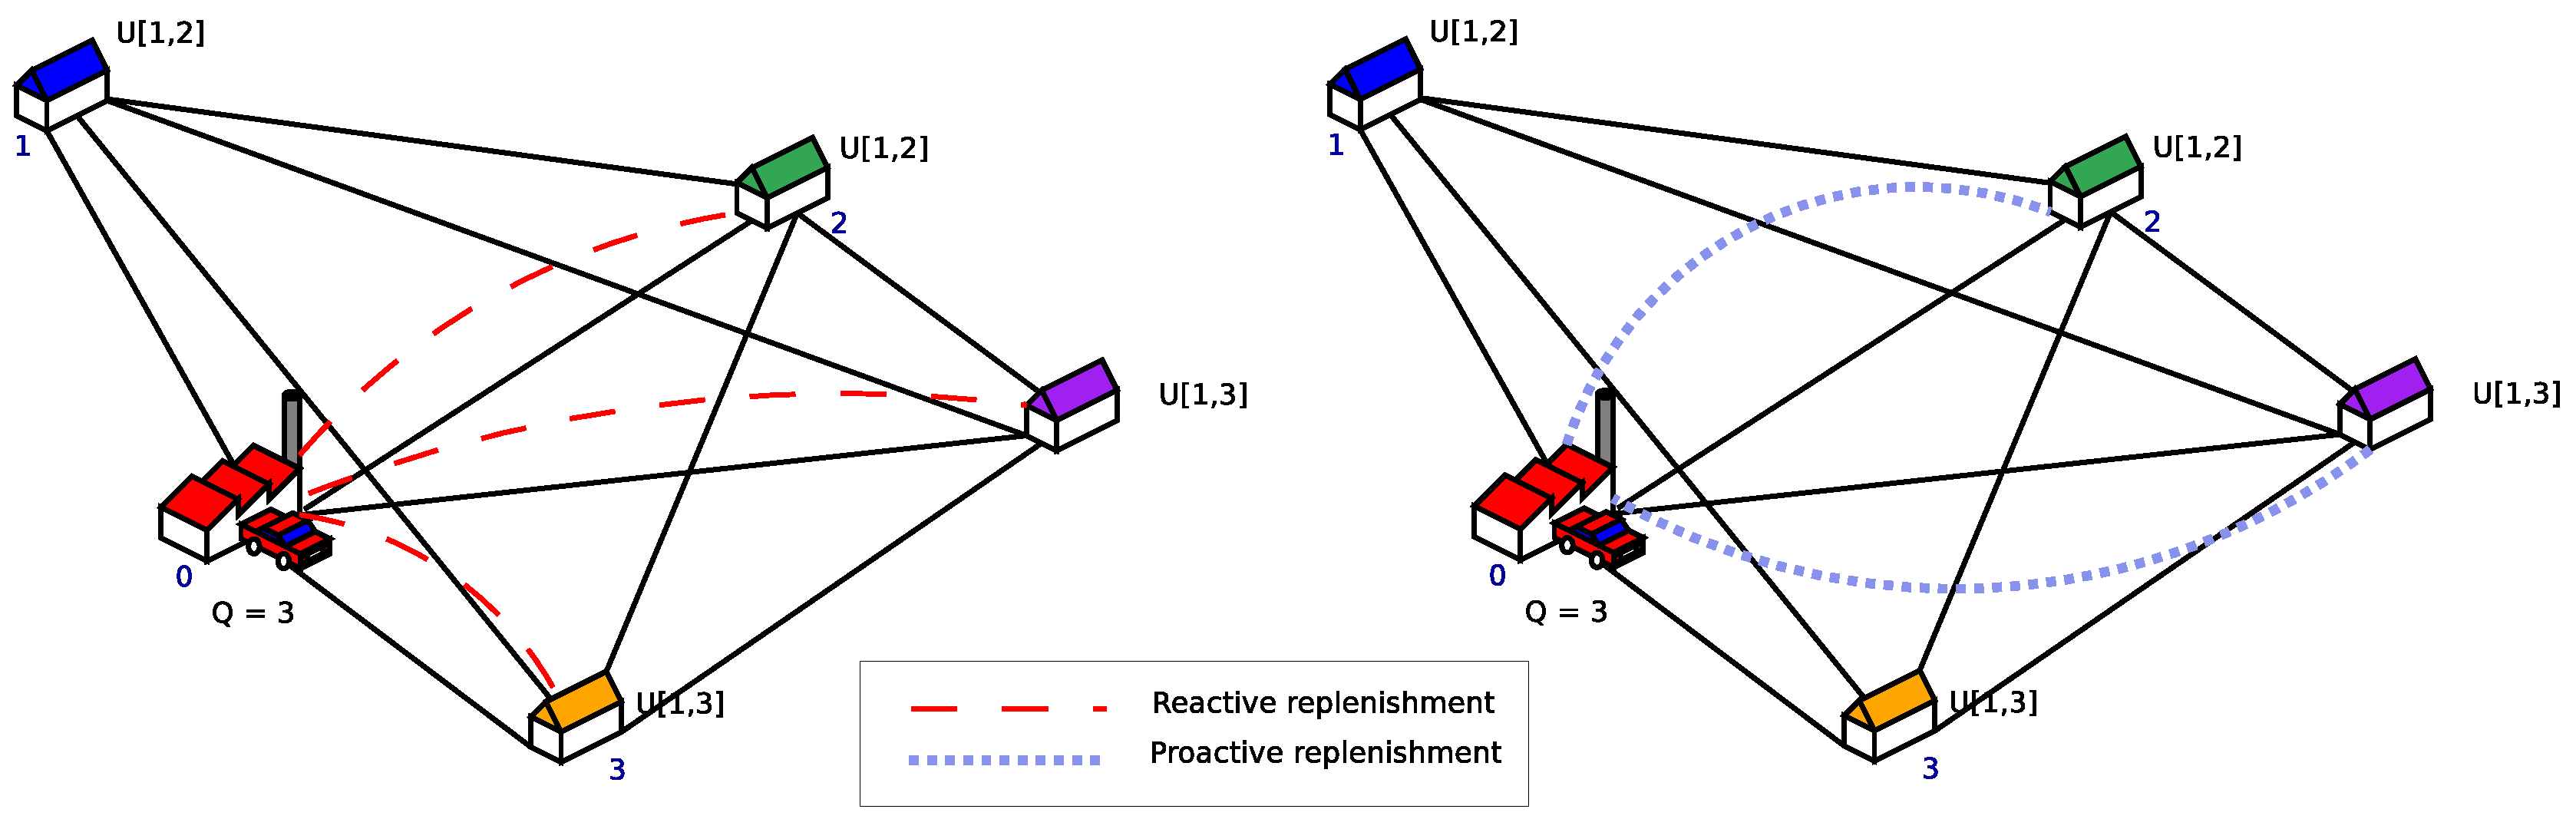
\includegraphics[width=1\textwidth]{Images/Chapter2/exIns4a.eps}
  \end{center}
    \caption{static and mixed routing policies}\label{fig:routing_policies}
\end{figure}

In order to represent the system state at stage $k$, the vector $x_k$ is defined as $x_k=(l,q_l, r_1,\ldots,r_n)$ of size $n+2$, where $l \in \{0,1,\ldots,n\}$, is the current location of the vehicle and $q_l \leq Q$ is its available capacity \textit{after} delivery to customer $l$; the elements $r_i$ represents the remaining demand to satisfy to the costumer $i$. An unknown demand is denoted as -, if customer $i$ is visited and its demand has been completely satisfied, $r_i$ will take the value 0; otherwise, it will take any value between 1 and $R$. The initial state of the system $x_0$ is $(0,Q,-,-,\ldots,-)$ and the final state $x_N$ occurs when the vehicle returns to the depot after serving the demands of customers, represented as $(0,Q,0,0,\ldots,0)$. Thus, the number of states in the system is $O(nQR^n)$

Let $N$ be a random variable representing the number of stages or transitions from initial state to the end, the vector $\pi = {\mu_0, \mu_1,\ldots, \mu_{N-1}}$ is the policy or sequence of functions to optimize, where $\mu_k$ is a function that associates a decision or control $u_k=\mu_k(x_k)$ for each state, $u_k \in U_k(x_k)$ and $U_k(x_k) = \{\{m \in \{1,\ldots,n\}\}|r_m\neq0\}\cup 0\} \times \{a:a \in \{0,1\}\}$. Control $u_k$ is represented as ordered pairs $(m,a)$, $m$ is any costumer not yet served, $m$ is 0 when all demands have been satisfied and the system enters its completion stage, $a$ is 0 if the vehicle directly visits customers and 1 if the vehicle first stops at the depot to resupply.

Given a state $x_k=(l,q_l,r_1,\ldots,r_m,\ldots,r_n)$ and a control $u_k$ in which it is decided to visit the node $m$ at the next stage, the random variable $D_m$ is realized ($r_m = D_m$ if $r_m$ is unknown; otherwise $r_m \neq ?$) and the remaining demand of the customer $m$ changes to $r'_m$ as soon as the capacity of vehicle becomes $q_m$, where

\begin{equation}\label{eq:q_m}
    q_m = \left \{ \begin{array}{ll}
    max(0,q_l-r_m), & \text{whether } u_k(m,0)=\mu_k(x_k)\\
    q_l+Q-r_m, & \text{whether } u_k(m,1)=\mu_k(x_k)
    \end{array} \right.
 \end{equation}

and

\begin{equation}\label{eq:r_m}
    r'_m = \left \{ \begin{array}{ll}
    min(0,r_m - q_l), & \text{whether } u_k(m,0)=\mu_k(x_k)\\
    0, & \text{whether } u_k(m,1)=\mu_k(x_k)
    \end{array} \right.
 \end{equation}

so the system goes to state $x_{k+1} = (m,q_m,r_1,\ldots,r'_m,\ldots,r_n)$. The transition between states is graphically represented as:

\begin{figure}[!htbp]
  \begin{center}
   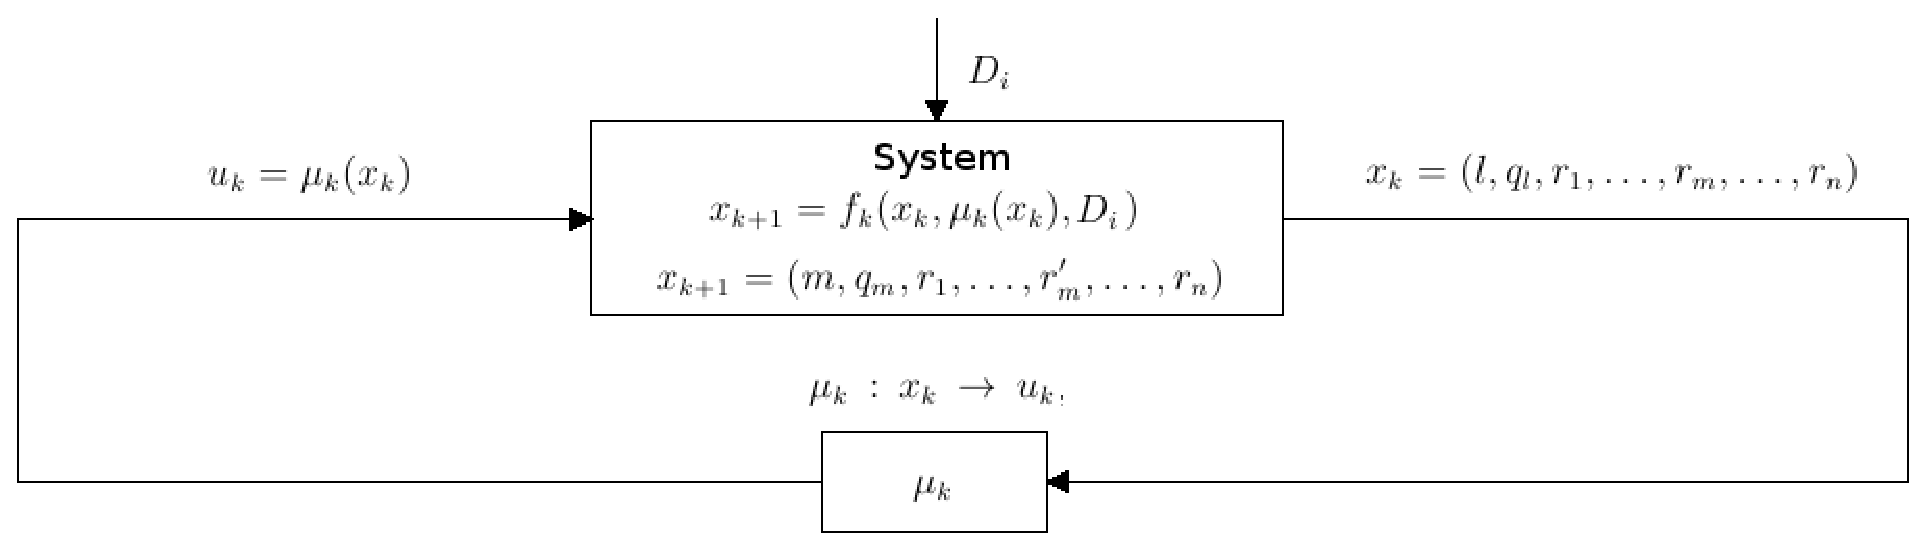
\includegraphics[width=1\textwidth]{Images/Chapter2/System_SDP.eps}
  \end{center}
    \caption{Stochastic Dynamic System for VRPSD}\label{fig:SDPS_VRPSD}
\end{figure}

Incurring in a transition cost $g(x_k,u_k,x_{k+1})$

\begin{equation}\label{eq:costg}
    g(x_k,\mu_k(x_k),x_{k+1}) = \left \{ \begin{array}{ll}
    d(l,m), & \text{whether } u_k(m,0)=\mu_k(x_k)\\
    d(l,0) + d(0,m), & \text{whether } u_k(m,1)=\mu_k(x_k)
    \end{array} \right.
 \end{equation}

The objective of the problem is to find a policy $\pi$ that minimizes the cost of transport $J_N^\pi$ (\ref{eq:SDP_obj_VRPSD}) in the $N$-stages or the expected cost to complete given an initial state. The optimal cost of transport in the $N$-stage $x$ is  $J_N^*(x) = min_{\pi\in \Pi}J_N^\pi(x)$, where $\Pi$ is the set of admissible policies. 

\begin{equation}\label{eq:SDP_obj_VRPSD}
 J_N^\pi(x_0)=E\biggr\{\sum_{k=0}^{N-1}g(x_k,\mu_k(x_k),x_{k+1})\biggr\}
\end{equation}

If $J_N^*(x)$ is known for all stages, the optimal control $u_k^*$ at each stage is to find the minimum of the following equation (\ref{eq:u_k^*}):

\begin{multline}\label{eq:u_k^*}
     u_k^*=\mu_k^*(x)=
\arg\min\limits_{u_k \in U_k(x_k)}g(x_k,u_k,x_{k+1})+\\
\sum_{x_{k+1}\in S}p_{x_kx_{k+1}}(u_k)J_N^*(x_{k+1})|x_k=x, \forall x\in S
\end{multline}

The problem is that $J_N^*(x)$ is unknown and its calculation is a computationally intractable problem given the size of state space. Secomandi ~\cite{secomandi_rollout_2001} points out that computing an optimal policy becomes quickly intractable when $n$ grows beyond 10. Chapter \ref{chap:dp_methodology} deals with issue of approximating this function through a dynamic-programming method efficiently computable.

\section{Summary}

The VRPSD has been studied for more than 20 years, with important progress in 90's and 00's and wide areas of application in logistics, following the conclusions of ~\cite{Dror_2005} the most promising approach is modeling the problem as a Markov decision process. Hence, a stochastic programming model is selected: a methodology for sequential decisions made under uncertainty, based on dynamic system, where the main idea is to use an approximate a function $J$ in order to make decisions in complex dynamic systems, allowing to deal with instances considered intractable for their size. In the next section, the dynamic programming solution is addressed.